The measured spectrum of a physical observable, like the jet mass distribution, is usually distorted by	detector effects, such as finite resolution and limited acceptance. Moreover, in this analysis the chosen bin size is comparable to the resolution, so there is a significant migration of events generated in one jet bin mass and ending up in a different bin of reconstructed jet mass. A comparison of the measured mass spectrum with that predicted at generator level requires that we remove these effects to obtain the true underlying mass spectrum. There are several possible ways to achieve the unfolding of detector effects on measured spectra, and examples can be found in \cite{unfold} and references therein. In this section we describe the unfolding method adopted in this analysis, which largely follows the technique proposed in \cite{agostini}. 
A physical quantity $\alpha$, distributed according to its probability density function $f(\alpha)$, cannot be measured perfectly. Apart from statistical uncertainties, there will be effects from reconstruction efficiency and finite resolution of the detector. As	a result, instead of the true, physical variable $\alpha$, a variable $\beta$, distributed according to some distribution $g(\beta)$, is measured. The relation between $f(\alpha)$ and $g(\beta)$ can be expressed as a convolution of the true distribution $f(\alpha)$ with a kernel $\hat{A}(\alpha,\beta)$ describing the detector effects,

\begin{equation}
\int f(\alpha) \hat{A}(\alpha,\beta)d\alpha = g(\beta)
\end{equation}

\noindent The spectrum we intend to unfold is given as an histogram. Hence, we use vectors and matrices for the formulation of the convolution,	

\begin{equation}
\hat{A} x = b
\label{eq:unf1}
\end{equation}

\noindent where the $i$-th component of the $n_x$-dimensional vector $x$ and the $n_b$-dimensional vector $b$ contain the number of entries in bin $i$ of the true and the measured distribution, respectively. 
$\hat{A}$ is a $(n_b - n_x)$-dimensional matrix, and contains the detector effects. An event with a true value in bin $j$ might be measured with a value in bin $i$ (i.e. finite resolution) or might not be measured at all. The matrix element $\hat{A}_{ij}$ represents the probability for an event	 with a true value in bin $x_j$ to be measured with a value in bin $b_i$.
Assuming that the measurement process is well simulated, $\hat{A}$ can be determined on Monte Carlo events by tracking the true and reconstructed values for each event. A well-defined system of linear equations is obtained,

\begin{equation}
\hat{A} x^{ini} = b^{ini}
\end{equation}


\noindent where the index ``ini''denotes the use of Monte Carlo spectra $x^{ini}$ , $b^{ini}$. Technically, the matrix element $\hat{A}_{ij}$ is determined by taking the number of events that fall into bin $j$ of $x^{ini}$ and at the same time into bin $i$ of $b^{ini}$, and by dividing this number by the number of events in bin $j$ of $x^{ini}$. The detector response matrix for the jet mass distribution is shown in Fig.~\ref{}, while in Fig. 34 we present the comparison between the generated  and the reconstructed jet mass distributions after all the selection criteria have been applied.

Now that $\hat{A}$ is determined and we have a measured spectrum $b$, one can try to solve Eq.~\ref{eq:unf1} for the true spectrum $x$. However, the apparently easiest way to determine $x$, i.e. applying $x = \hat{A}^{-1}b$, is not adequate. Even when $\hat{A}$ can be inverted, statistical fluctuations in the measured spectrum introduce spurious, non-physical oscillations in the solution for $x$. Therefore a more efficient method needs to be applied. 

We use an unfolding procedure described by G.~D.~Agostini in~\cite{agostini}. Repeated application of Bayes theorem is used to invert the response matrix. Regularization is achieved by stopping iterations before reaching the ``true'' (but wildly fluctuating) inverse. The regularization parameter is just the number of iterations.
 In principle, this has to be tuned to prevent the statistical fluctuations being interpreted as structure in the true distribution, according to the sample statistics and binning. In practice, the results are fairly insensitive to the precise setting used and four iterations are usually sufficient.
The training truth is taken as its initial prior, rather than a flat distribution. This should not bias result once we have iterated, but could reach an optimum after fewer iterations.
This implementation takes account of errors on the data sample but not, by default, uncertainties in the response matrix due to finite MC statistics. That calculation can be very slow, and usually the training sample is much larger than the data sample.
%RooUnfoldBayes does not normally do smoothing, since this has not been found to be necessary 2
%and can, in principle, bias the distribution. Smoothing can be enabled with an option.


The detector response matrix for the different jet clustering algorithms are showed in Fig.~\ref{figs:unfo2d_1}-\ref{figs:unfo2d_4}. We show the response in the 4 nominal $p_T$ bins used for the analysis, for the AK7 jets with the following clustering algorithm: ungroomed, pruned, filtered and trimmed.

\begin{figure}[!htb]
\centering
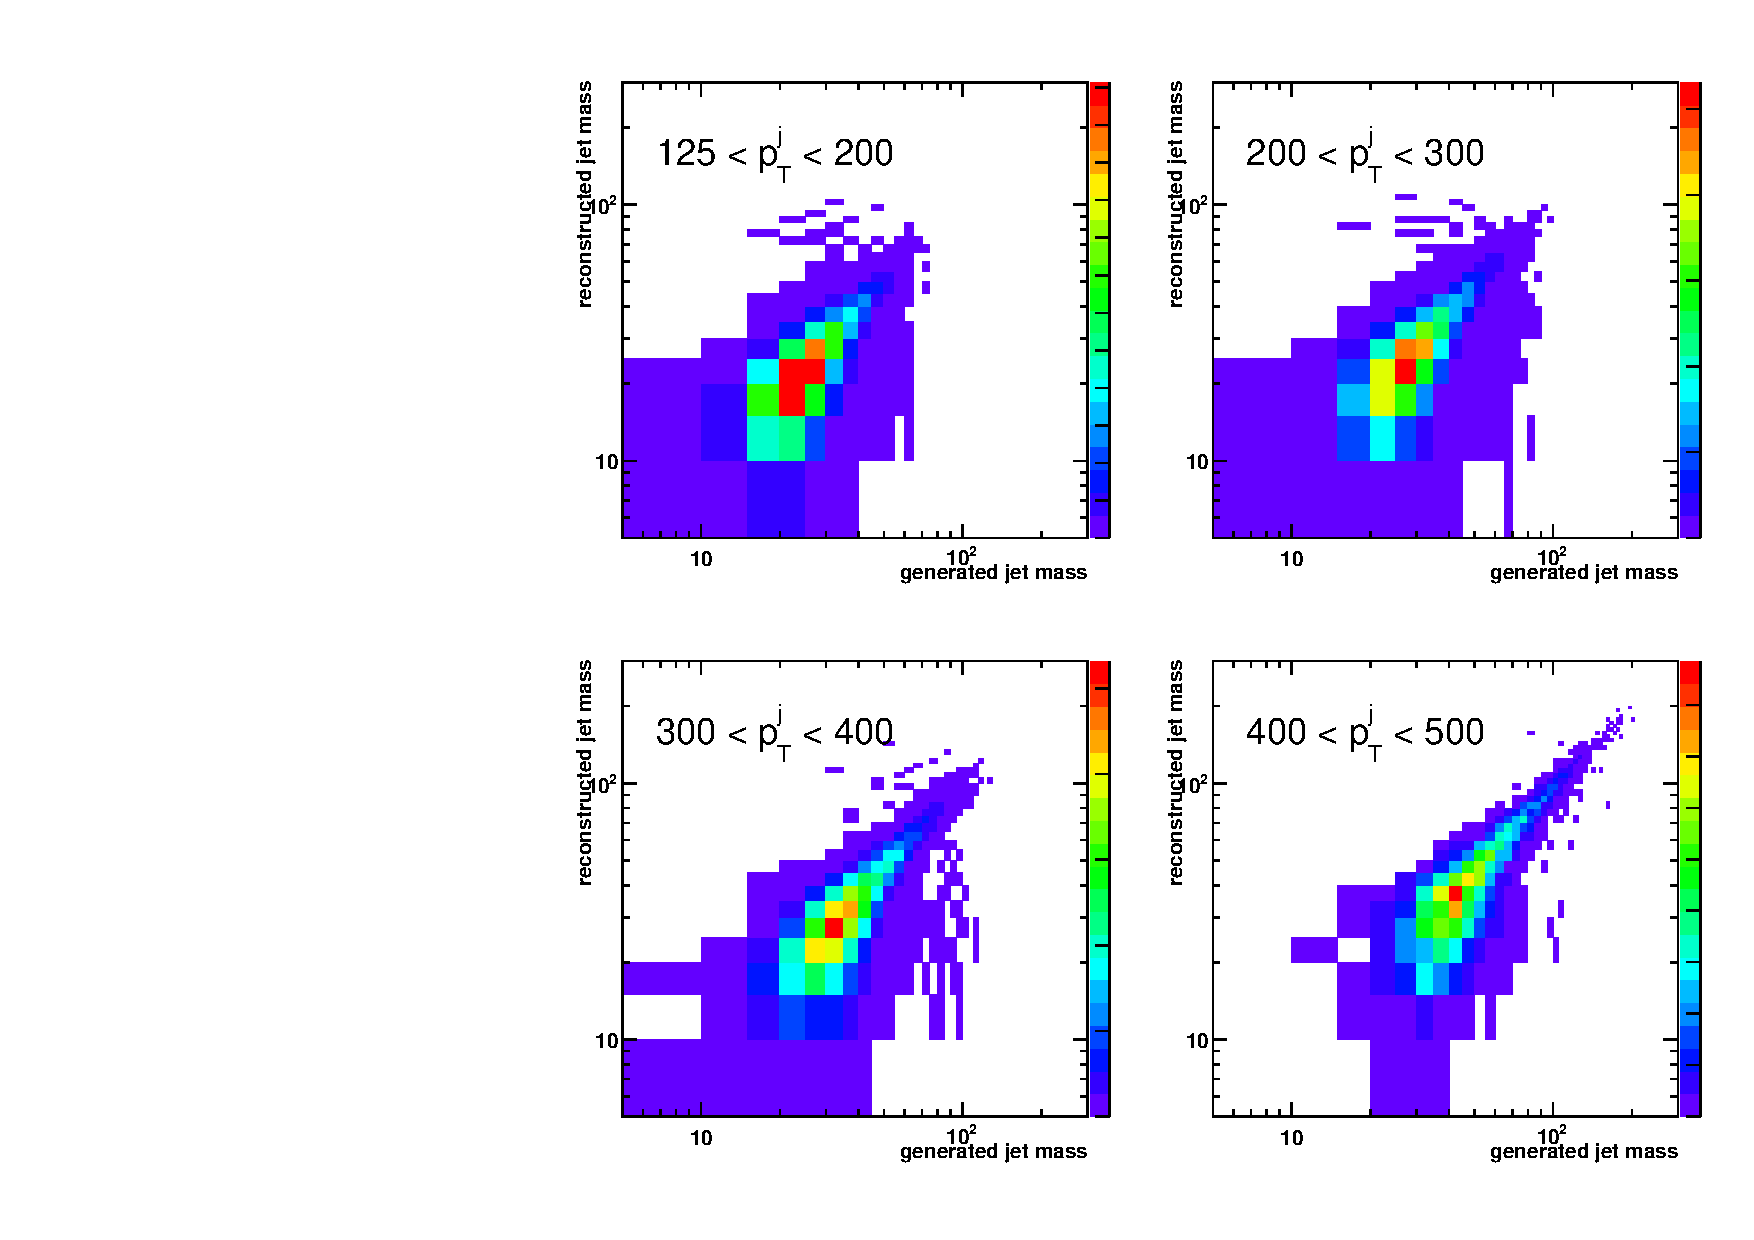
\includegraphics[width=1.0\textwidth]{figs/unf_response_ak7_pTbins.pdf}
\caption{Detector response matrix for ungroomed AK7 jets for various $p_T$ bins. The true jet 
mass is shown on the $x$-axis, and the reconstructed jet mass is shown on the $y$-axis, using the Madgraph generator.}
\label{figs:unfo2d_1}
\end{figure}

\begin{figure}[!htb]
\centering
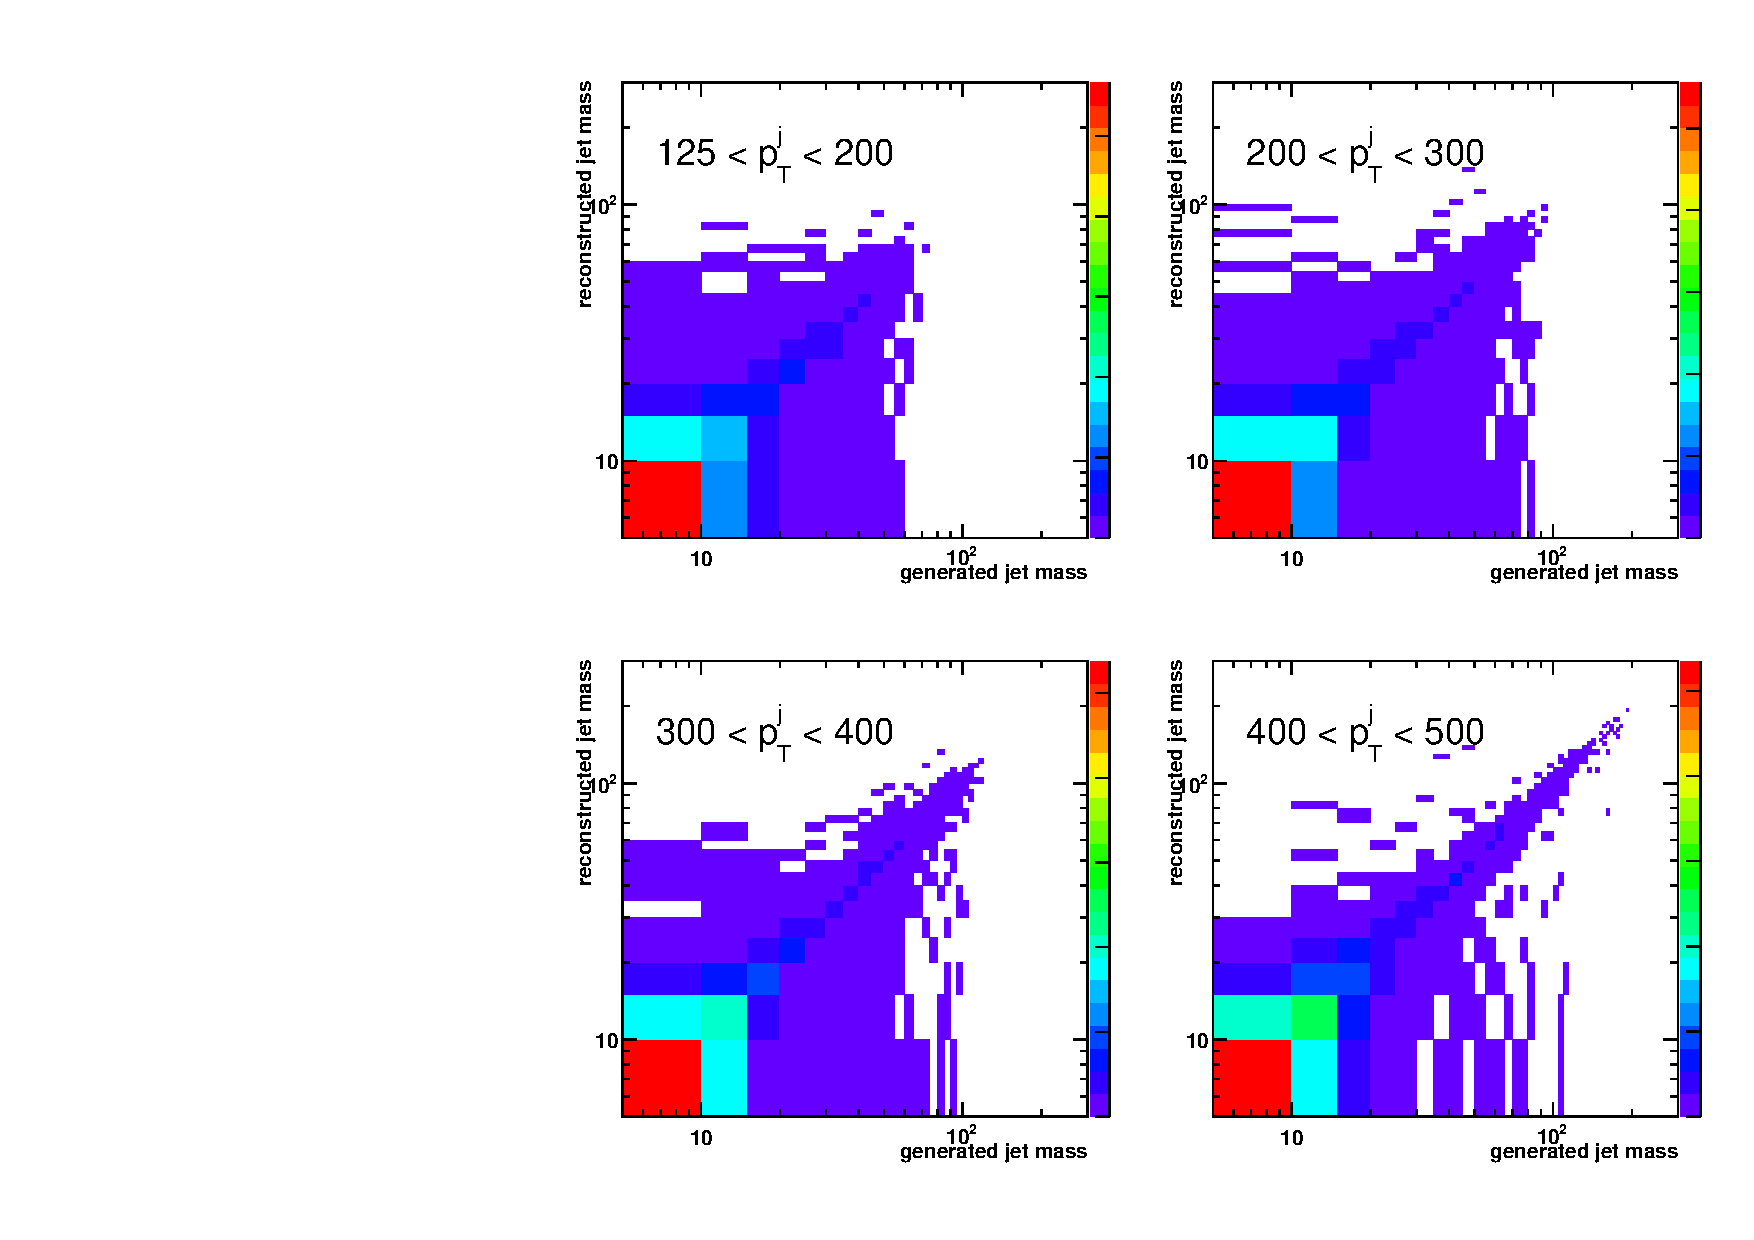
\includegraphics[width=1.0\textwidth]{figs/unf_response_ak7pr_pTbins.pdf}
\caption{Detector response matrix for groomed AK7 pruned jets for various $p_T$ bins. The true jet 
mass is shown on the $x$-axis, and the reconstructed jet mass is shown on the $y$-axis, using the Madgraph generator.}
\label{figs:unfo2d_2}
\end{figure}

\begin{figure}[!htb]
\centering
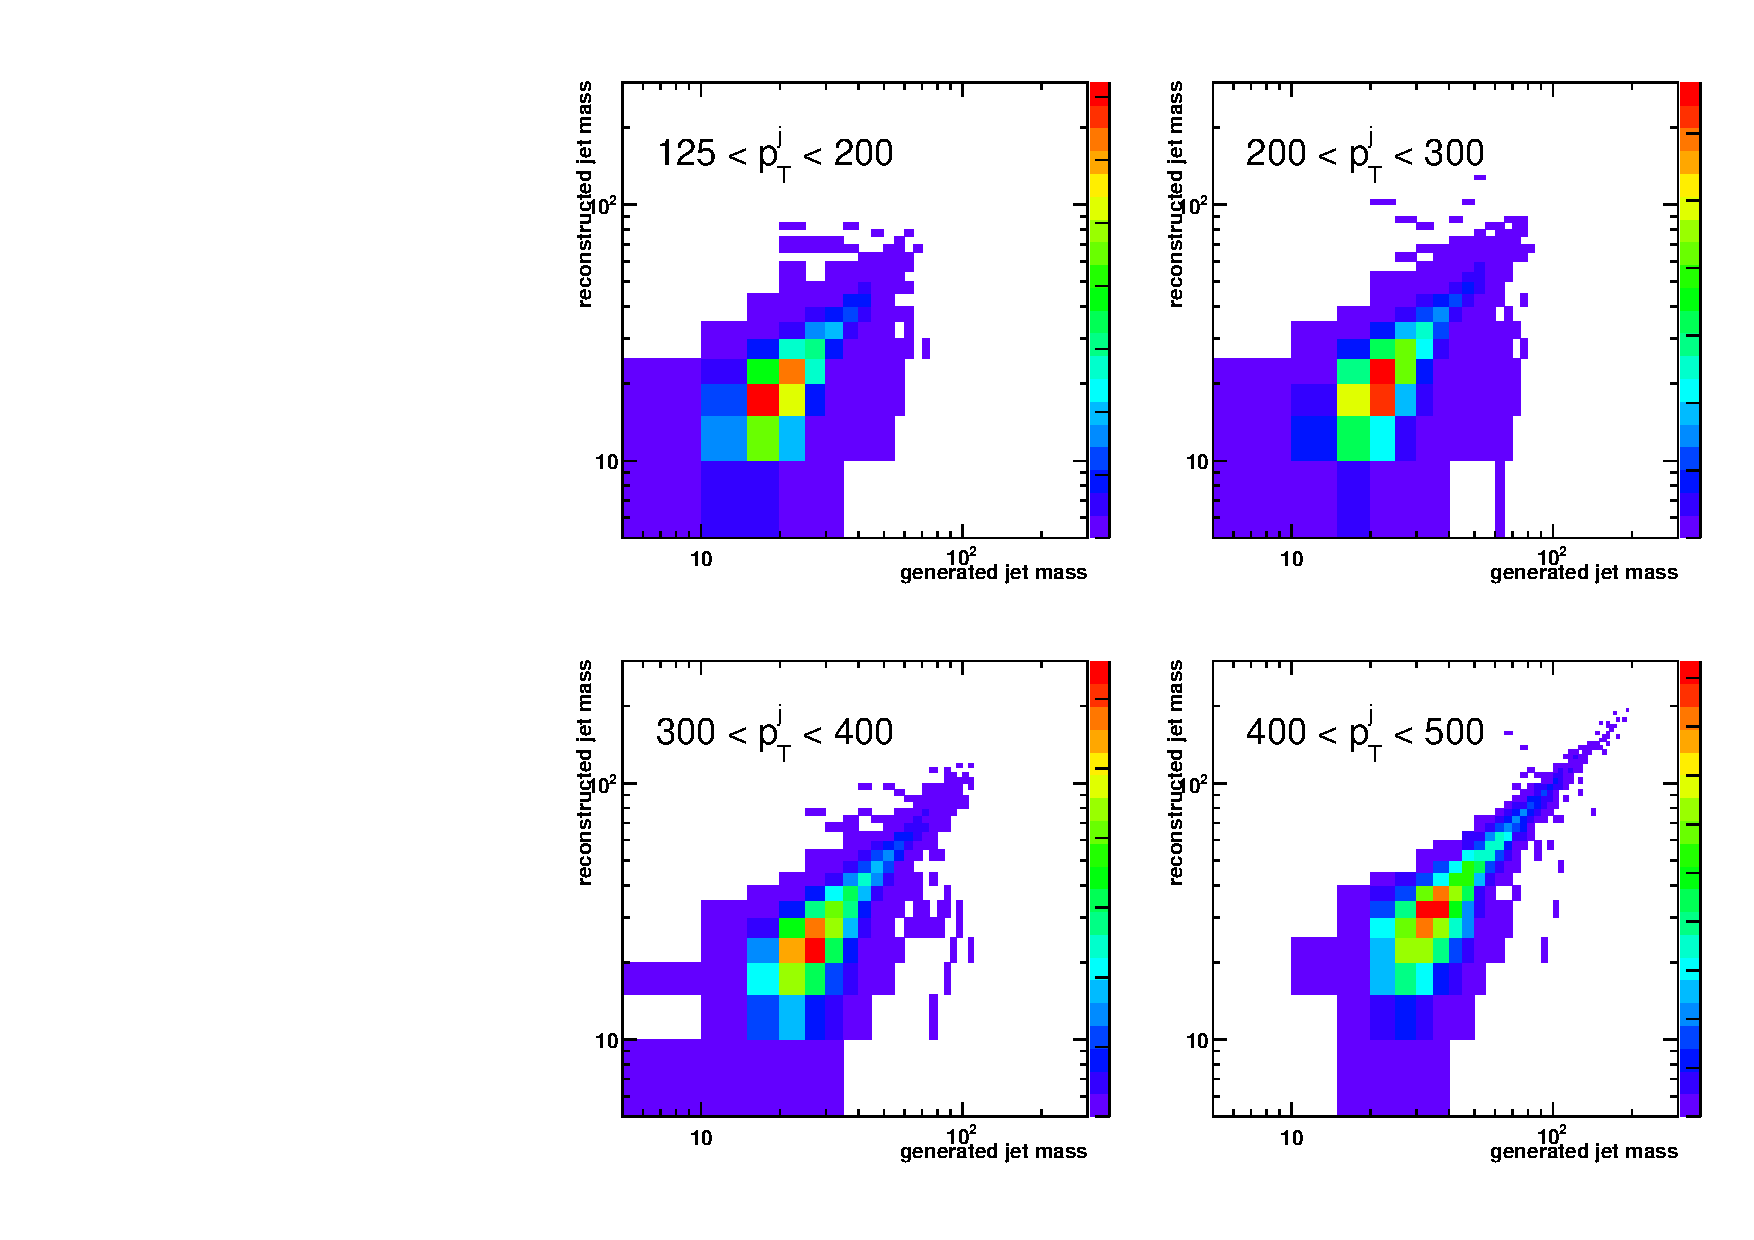
\includegraphics[width=1.0\textwidth]{figs/unf_response_ak7ft_pTbins.pdf}
\caption{Detector response matrix for groomed AK7 filtered jets for various $p_T$ bins. The true jet 
mass is shown on the $x$-axis, and the reconstructed jet mass is shown on the $y$-axis, using the Madgraph generator.}
\label{figs:unfo2d_3}
\end{figure}

\begin{figure}[!htb]
\centering
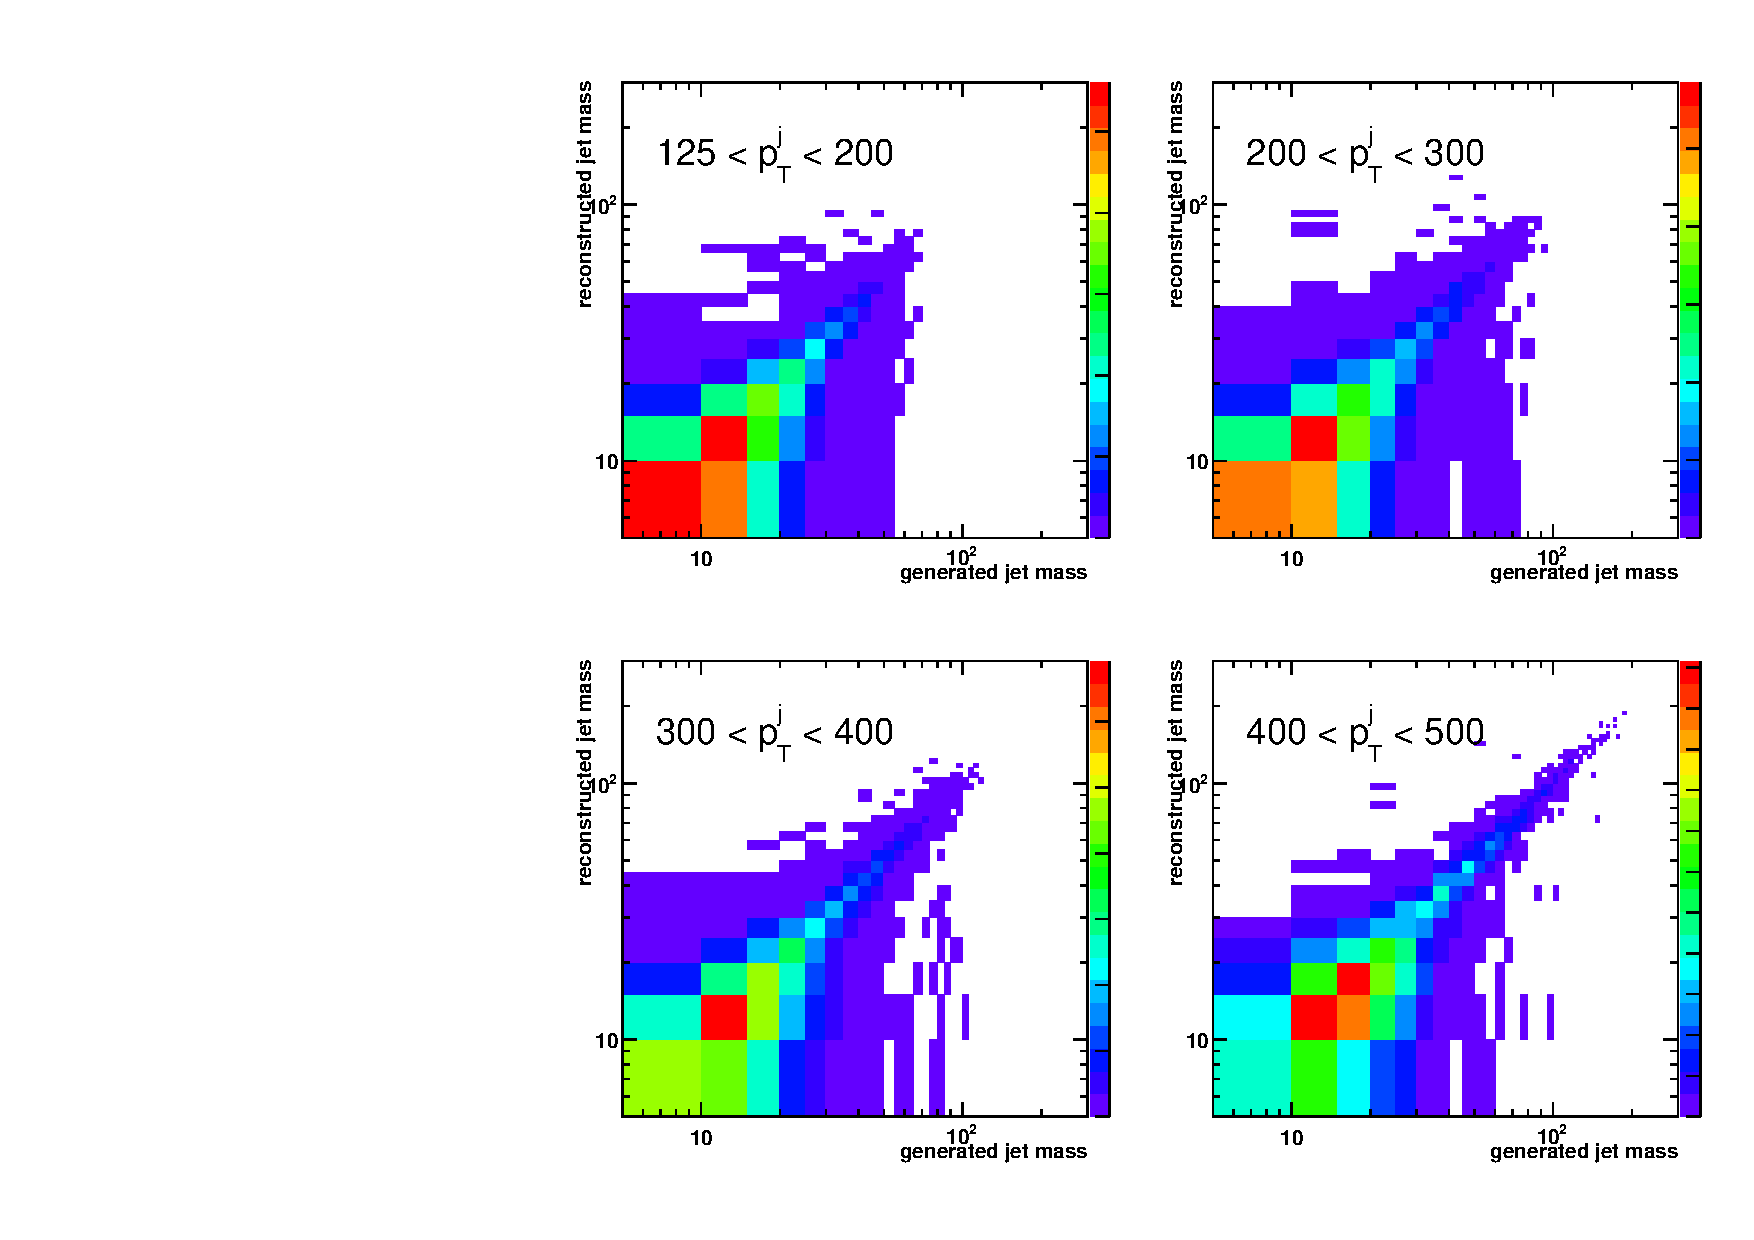
\includegraphics[width=1.0\textwidth]{figs/unf_response_ak7tr_pTbins.pdf}
\caption{Detector response matrix for groomed AK7 trimmed jets for various $p_T$ bins. The true jet 
mass is shown on the $x$-axis, and the reconstructed jet mass is shown on the $y$-axis, using the Madgraph generator.}
\label{figs:unfo2d_4}
\end{figure}


We validate the unfolding procedure on MC events in the following way: we use one half of the MC to build the detector response matrix and use the second half as it was ``data'' to perform the unfolding procedure and compare with the true jet mass spectrum. An example of such closure test for ungroomed AK7 jets is shown in Fig.~\ref{figs:closure}.

\begin{figure}[!htb]
\centering
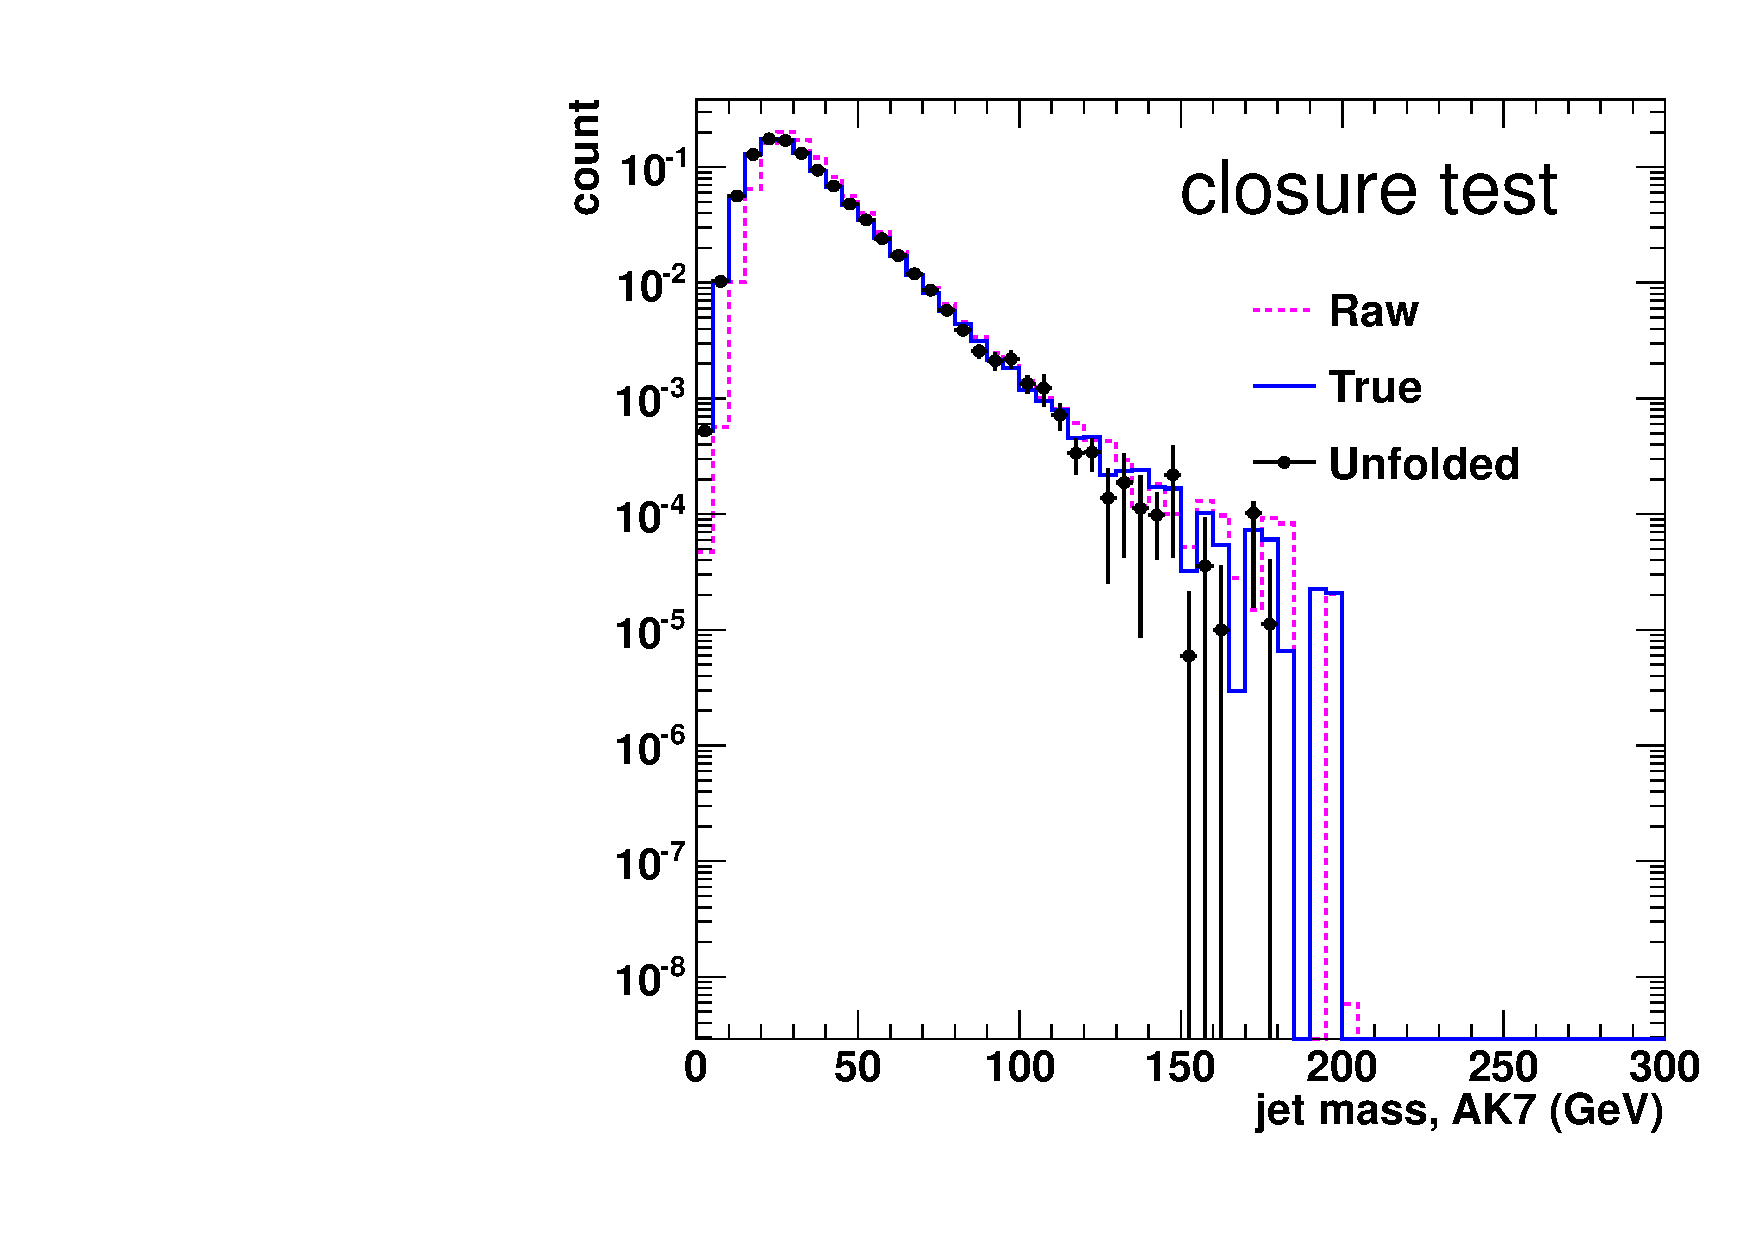
\includegraphics[width=1.0\textwidth]{figs/closureTest_ak7.pdf}
\caption{Unfolding closure test: unfolded jet mass distribution for ungroomed AK7 jet in MC events compared with the true level one, using a detector response matrix built on independent MC events.}
\label{figs:closure}
\end{figure}


~                                                                                                                           



